\subsection{สนามแม่เหล็กและเส้นสนามแม่เหล็ก}
\begin{minipage}{.5\textwidth}
\textbf{แม่เหล็ก (magnet)}  คือวัตถุที่ดูดเหล็กได้ และวัตถุที่แม่เหล็กส่งแรงกระทำเรียกว่า {\color{red} สารแม่เหล็ก (magnetic  substance)} 
\\\\
แท่งแม่เหล็ก 1 แท่งจะมี  2  ขั้วคือ \hfill ขั้วเหนือและ \\ ขั้วใต้ ขั้วแม่เหล็กชนิดเดียวกันจะผลักกันและขั้วต่างกันจะดูดกันเสมอ
\end{minipage} \hfill
\begin{adjustbox}{valign=c} 
    \begin{minipage}[c]{.45\linewidth}
        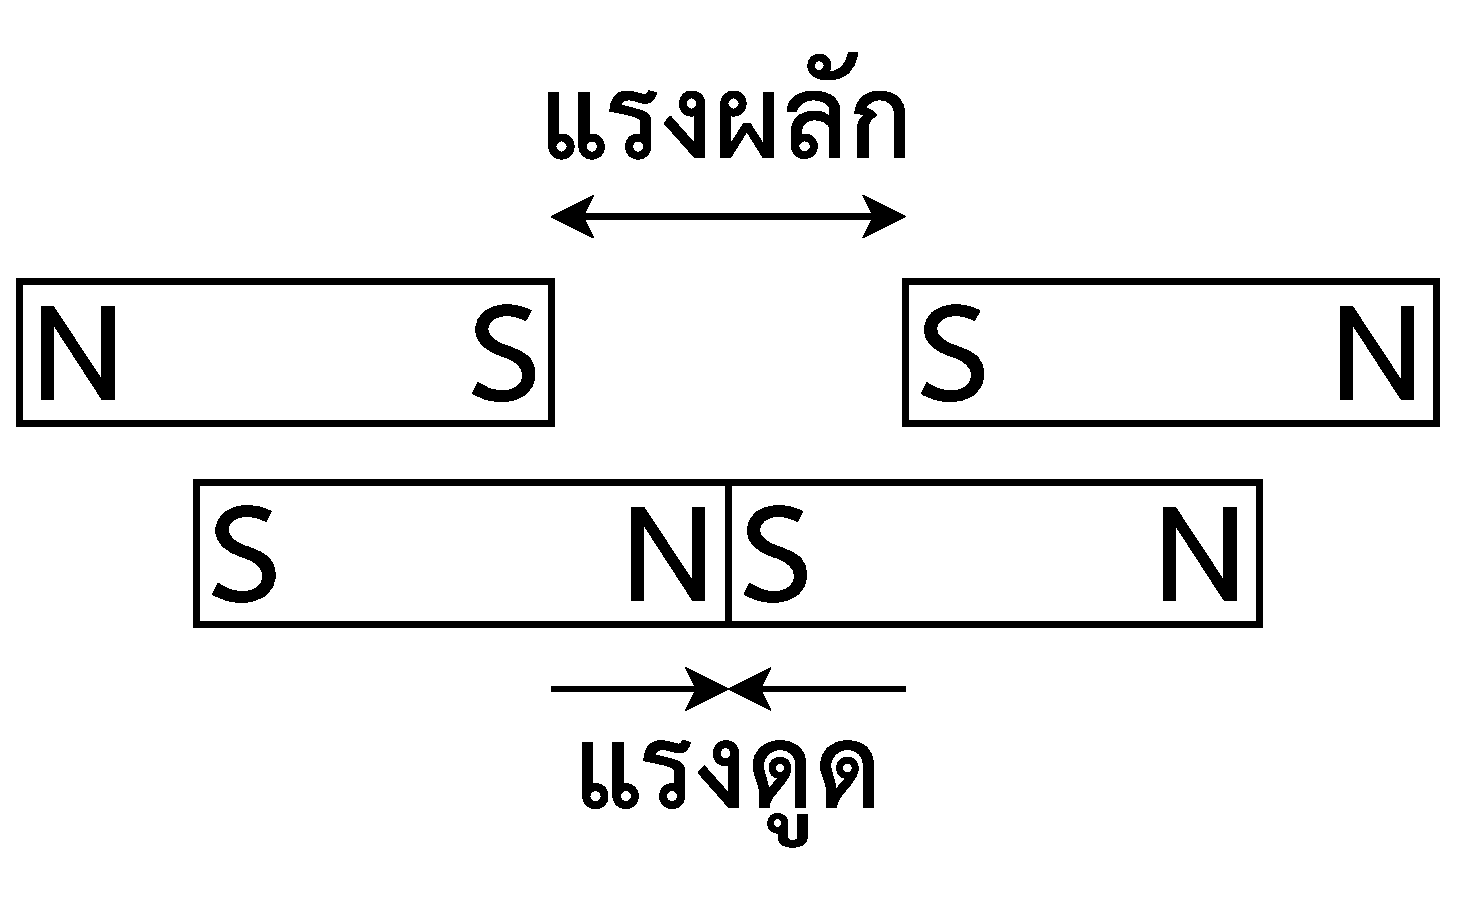
\includegraphics[width=\linewidth]{lesson2-1-1.eps}
    \end{minipage}
\end{adjustbox}

\tcblower

\begin{minipage}{.5\textwidth}
เมื่อวางแท่งแม่เหล็กลงบนแผ่นกระดาษ  แล้วโปรยผงเหล็กลงไป  จะพบว่า  แท่งแม่เหล็ก \hfill จะมีแรงกระทำต่อผงเหล็กเหล่านั้น  บริเวณที่มีแรงกระทำต่อผงเหล็กเรียกว่า \hfill {\color{red} สนามแม่เหล็ก (magnetic  field)}  \hfill      และแรงกระทำนี้จะทำให้ผงเหล็กเรียงตัวเป็นแนวเรียกแนวนี้ว่า {\color{red} \hfill เส้นสนามแม่เหล็ก  (magnetic  field  line)}
\end{minipage} \hfill
\begin{adjustbox}{valign=c} 
    \begin{minipage}[c]{.45\linewidth}
        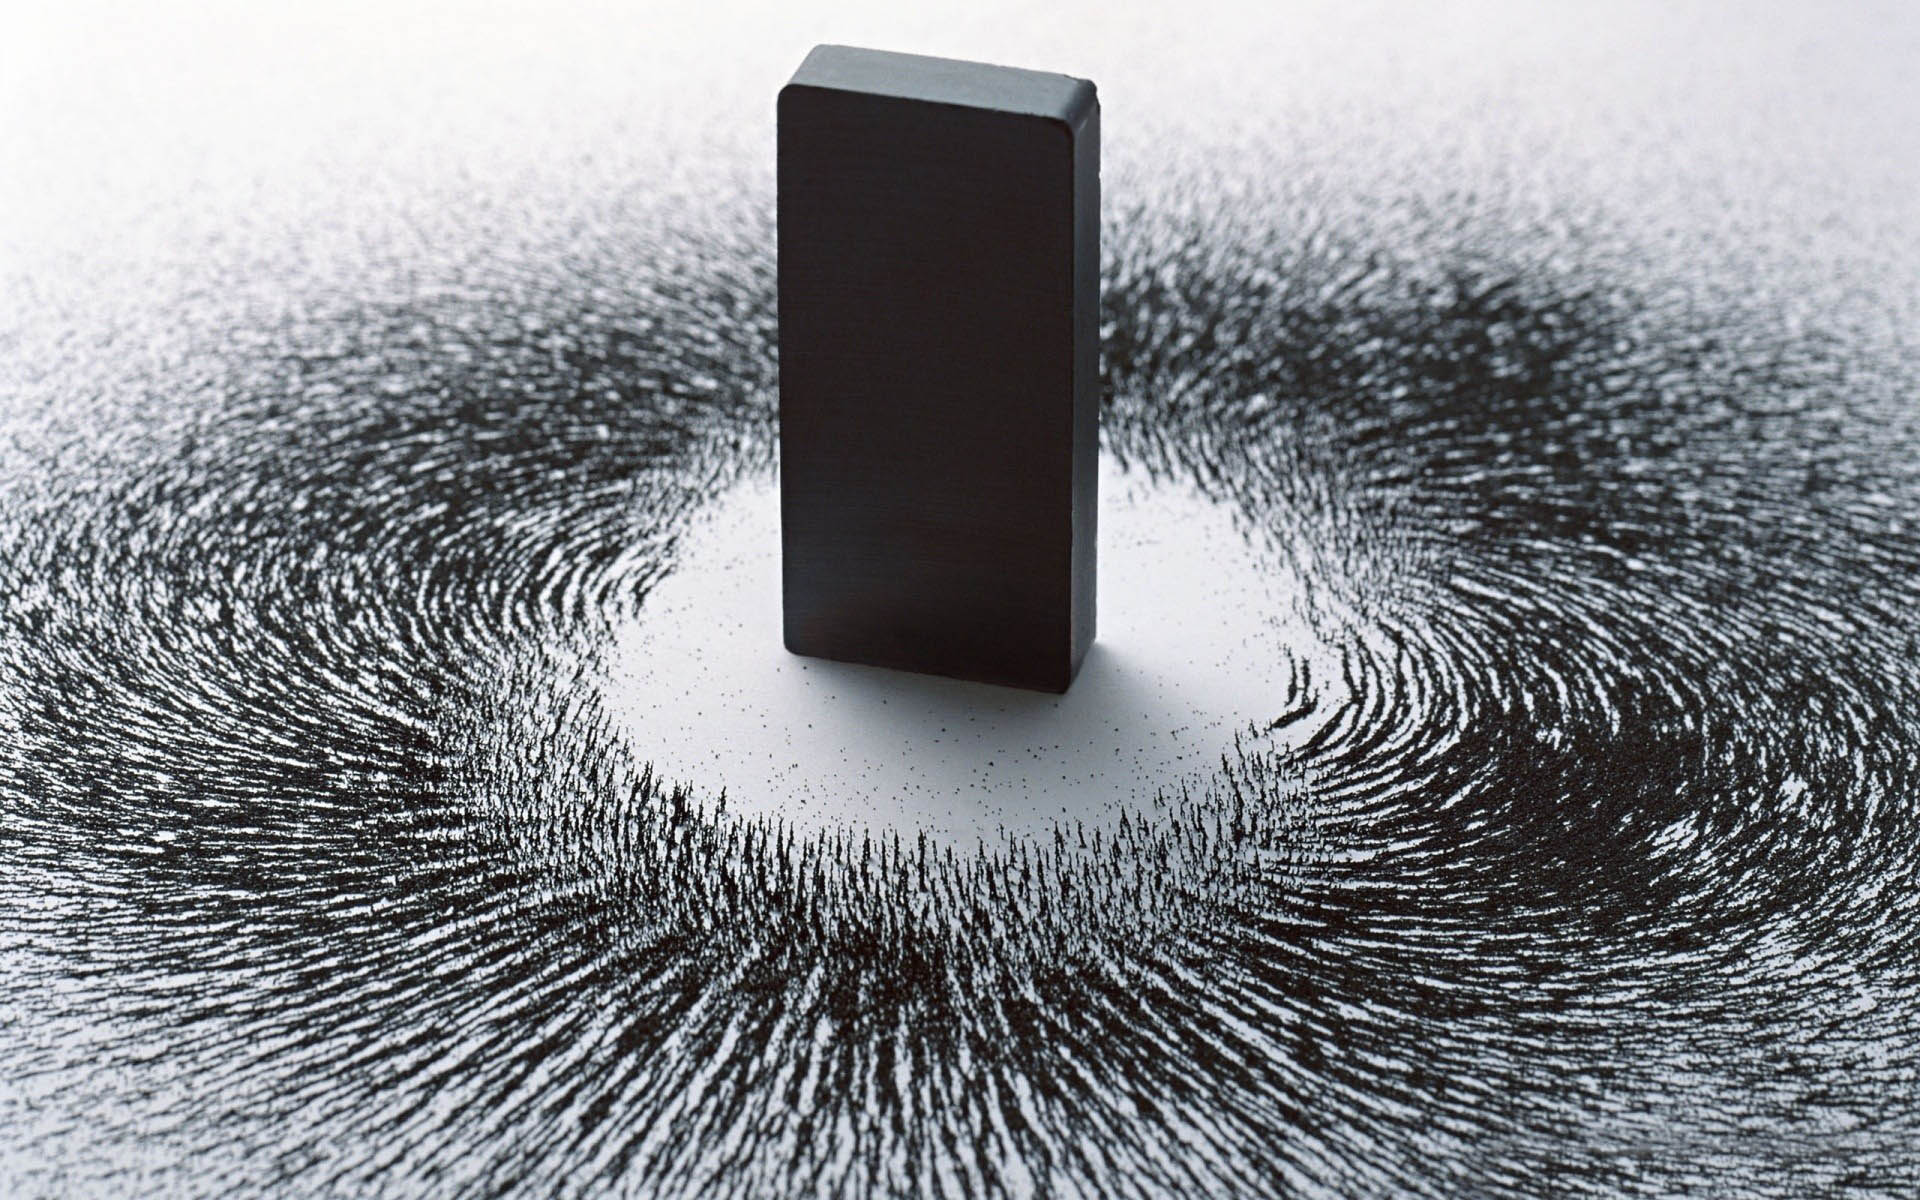
\includegraphics[width=\linewidth]{lesson2-1-1.jpg}
    \end{minipage}
\end{adjustbox}
